% Options for packages loaded elsewhere
\PassOptionsToPackage{unicode}{hyperref}
\PassOptionsToPackage{hyphens}{url}
%
\documentclass[
  ignorenonframetext,
]{beamer}
\usepackage{pgfpages}
\setbeamertemplate{caption}[numbered]
\setbeamertemplate{caption label separator}{: }
\setbeamercolor{caption name}{fg=normal text.fg}
\beamertemplatenavigationsymbolsempty
% Prevent slide breaks in the middle of a paragraph
\widowpenalties 1 10000
\raggedbottom
\setbeamertemplate{part page}{
  \centering
  \begin{beamercolorbox}[sep=16pt,center]{part title}
    \usebeamerfont{part title}\insertpart\par
  \end{beamercolorbox}
}
\setbeamertemplate{section page}{
  \centering
  \begin{beamercolorbox}[sep=12pt,center]{part title}
    \usebeamerfont{section title}\insertsection\par
  \end{beamercolorbox}
}
\setbeamertemplate{subsection page}{
  \centering
  \begin{beamercolorbox}[sep=8pt,center]{part title}
    \usebeamerfont{subsection title}\insertsubsection\par
  \end{beamercolorbox}
}
\AtBeginPart{
  \frame{\partpage}
}
\AtBeginSection{
  \ifbibliography
  \else
    \frame{\sectionpage}
  \fi
}
\AtBeginSubsection{
  \frame{\subsectionpage}
}
\usepackage{amsmath,amssymb}
\usepackage{lmodern}
\usepackage{ifxetex,ifluatex}
\ifnum 0\ifxetex 1\fi\ifluatex 1\fi=0 % if pdftex
  \usepackage[T1]{fontenc}
  \usepackage[utf8]{inputenc}
  \usepackage{textcomp} % provide euro and other symbols
\else % if luatex or xetex
  \usepackage{unicode-math}
  \defaultfontfeatures{Scale=MatchLowercase}
  \defaultfontfeatures[\rmfamily]{Ligatures=TeX,Scale=1}
\fi
\usetheme[]{Copenhagen}
\usecolortheme{dolphin}
\usefonttheme{structurebold}
% Use upquote if available, for straight quotes in verbatim environments
\IfFileExists{upquote.sty}{\usepackage{upquote}}{}
\IfFileExists{microtype.sty}{% use microtype if available
  \usepackage[]{microtype}
  \UseMicrotypeSet[protrusion]{basicmath} % disable protrusion for tt fonts
}{}
\makeatletter
\@ifundefined{KOMAClassName}{% if non-KOMA class
  \IfFileExists{parskip.sty}{%
    \usepackage{parskip}
  }{% else
    \setlength{\parindent}{0pt}
    \setlength{\parskip}{6pt plus 2pt minus 1pt}}
}{% if KOMA class
  \KOMAoptions{parskip=half}}
\makeatother
\usepackage{xcolor}
\IfFileExists{xurl.sty}{\usepackage{xurl}}{} % add URL line breaks if available
\IfFileExists{bookmark.sty}{\usepackage{bookmark}}{\usepackage{hyperref}}
\hypersetup{
  pdftitle={Application of Hypothesis Tests},
  pdfauthor={Alex Sanchez, Miriam Mota and Santiago Perez-Hoyos},
  hidelinks,
  pdfcreator={LaTeX via pandoc}}
\urlstyle{same} % disable monospaced font for URLs
\newif\ifbibliography
\usepackage{color}
\usepackage{fancyvrb}
\newcommand{\VerbBar}{|}
\newcommand{\VERB}{\Verb[commandchars=\\\{\}]}
\DefineVerbatimEnvironment{Highlighting}{Verbatim}{commandchars=\\\{\}}
% Add ',fontsize=\small' for more characters per line
\usepackage{framed}
\definecolor{shadecolor}{RGB}{248,248,248}
\newenvironment{Shaded}{\begin{snugshade}}{\end{snugshade}}
\newcommand{\AlertTok}[1]{\textcolor[rgb]{0.94,0.16,0.16}{#1}}
\newcommand{\AnnotationTok}[1]{\textcolor[rgb]{0.56,0.35,0.01}{\textbf{\textit{#1}}}}
\newcommand{\AttributeTok}[1]{\textcolor[rgb]{0.77,0.63,0.00}{#1}}
\newcommand{\BaseNTok}[1]{\textcolor[rgb]{0.00,0.00,0.81}{#1}}
\newcommand{\BuiltInTok}[1]{#1}
\newcommand{\CharTok}[1]{\textcolor[rgb]{0.31,0.60,0.02}{#1}}
\newcommand{\CommentTok}[1]{\textcolor[rgb]{0.56,0.35,0.01}{\textit{#1}}}
\newcommand{\CommentVarTok}[1]{\textcolor[rgb]{0.56,0.35,0.01}{\textbf{\textit{#1}}}}
\newcommand{\ConstantTok}[1]{\textcolor[rgb]{0.00,0.00,0.00}{#1}}
\newcommand{\ControlFlowTok}[1]{\textcolor[rgb]{0.13,0.29,0.53}{\textbf{#1}}}
\newcommand{\DataTypeTok}[1]{\textcolor[rgb]{0.13,0.29,0.53}{#1}}
\newcommand{\DecValTok}[1]{\textcolor[rgb]{0.00,0.00,0.81}{#1}}
\newcommand{\DocumentationTok}[1]{\textcolor[rgb]{0.56,0.35,0.01}{\textbf{\textit{#1}}}}
\newcommand{\ErrorTok}[1]{\textcolor[rgb]{0.64,0.00,0.00}{\textbf{#1}}}
\newcommand{\ExtensionTok}[1]{#1}
\newcommand{\FloatTok}[1]{\textcolor[rgb]{0.00,0.00,0.81}{#1}}
\newcommand{\FunctionTok}[1]{\textcolor[rgb]{0.00,0.00,0.00}{#1}}
\newcommand{\ImportTok}[1]{#1}
\newcommand{\InformationTok}[1]{\textcolor[rgb]{0.56,0.35,0.01}{\textbf{\textit{#1}}}}
\newcommand{\KeywordTok}[1]{\textcolor[rgb]{0.13,0.29,0.53}{\textbf{#1}}}
\newcommand{\NormalTok}[1]{#1}
\newcommand{\OperatorTok}[1]{\textcolor[rgb]{0.81,0.36,0.00}{\textbf{#1}}}
\newcommand{\OtherTok}[1]{\textcolor[rgb]{0.56,0.35,0.01}{#1}}
\newcommand{\PreprocessorTok}[1]{\textcolor[rgb]{0.56,0.35,0.01}{\textit{#1}}}
\newcommand{\RegionMarkerTok}[1]{#1}
\newcommand{\SpecialCharTok}[1]{\textcolor[rgb]{0.00,0.00,0.00}{#1}}
\newcommand{\SpecialStringTok}[1]{\textcolor[rgb]{0.31,0.60,0.02}{#1}}
\newcommand{\StringTok}[1]{\textcolor[rgb]{0.31,0.60,0.02}{#1}}
\newcommand{\VariableTok}[1]{\textcolor[rgb]{0.00,0.00,0.00}{#1}}
\newcommand{\VerbatimStringTok}[1]{\textcolor[rgb]{0.31,0.60,0.02}{#1}}
\newcommand{\WarningTok}[1]{\textcolor[rgb]{0.56,0.35,0.01}{\textbf{\textit{#1}}}}
\usepackage{graphicx}
\makeatletter
\def\maxwidth{\ifdim\Gin@nat@width>\linewidth\linewidth\else\Gin@nat@width\fi}
\def\maxheight{\ifdim\Gin@nat@height>\textheight\textheight\else\Gin@nat@height\fi}
\makeatother
% Scale images if necessary, so that they will not overflow the page
% margins by default, and it is still possible to overwrite the defaults
% using explicit options in \includegraphics[width, height, ...]{}
\setkeys{Gin}{width=\maxwidth,height=\maxheight,keepaspectratio}
% Set default figure placement to htbp
\makeatletter
\def\fps@figure{htbp}
\makeatother
\setlength{\emergencystretch}{3em} % prevent overfull lines
\providecommand{\tightlist}{%
  \setlength{\itemsep}{0pt}\setlength{\parskip}{0pt}}
\setcounter{secnumdepth}{-\maxdimen} % remove section numbering
\ifluatex
  \usepackage{selnolig}  % disable illegal ligatures
\fi

\title{Application of Hypothesis Tests}
\author{Alex Sanchez, Miriam Mota and Santiago Perez-Hoyos}
\date{Versión 2022-02-14}
\institute{Statistics and Bioinformatics Unit. Vall d'Hebron Institut de
Recerca}

\begin{document}
\frame{\titlepage}

\begin{frame}{Outline}
\protect\hypertarget{outline}{}
\begin{enumerate}
\tightlist
\item
  INTRODUCTION. TYPES OF TESTS
\item
  NORMALITY TESTS
\item
  ONE GROUP COMPARISON
\item
  TWO GROUPS COMPARISON IN INDEPENDENT / DEPENDENT SAMPLES
\item
  CATEGORICAL VARIABLES
\item
  PROPORTION TESTS
\item
  INDEPENDENCE TESTS
\end{enumerate}
\end{frame}

\begin{frame}{Introduction}
\protect\hypertarget{introduction}{}
\begin{itemize}
\tightlist
\item
  Once the concept of hypothesis testing is established,
\item
  Researchers face the problem of \emph{which test should be applied at
  every possible situation}.
\item
  Best solution:

  \begin{itemize}
  \tightlist
  \item
    understand the problem and the questions addressed
  \item
    know available tests for each problem
  \item
    be aware of applicability assumptions of each test and how to check
    them.
  \end{itemize}
\item
  Easier to say than to do.

  \begin{itemize}
  \tightlist
  \item
    Sometimes cheatsheets may be helpful,
  \item
    but be warned against a blind use, that is:
  \item
    \textbf{understand} and \textbf{be critic} with the steps.
  \end{itemize}
\end{itemize}
\end{frame}

\begin{frame}{Select the test according to each situation (1)}
\protect\hypertarget{select-the-test-according-to-each-situation-1}{}
\begin{block}{Some test options when variables are numerical}
\protect\hypertarget{some-test-options-when-variables-are-numerical}{}
\begin{figure}
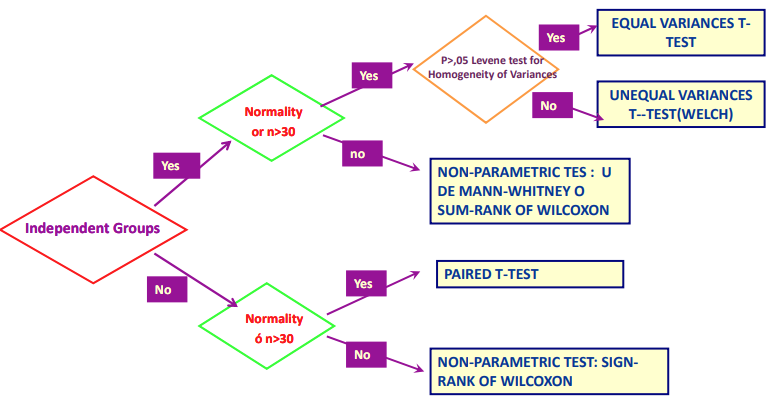
\includegraphics[width=0.8\linewidth,height=1\textheight]{images/tests4numericalVariables} \end{figure}
\end{block}
\end{frame}

\begin{frame}{Introductory Example}
\protect\hypertarget{introductory-example}{}
\begin{itemize}
\tightlist
\item
  A study was designed to compare two distinct hypertension control
  programs.
\item
  60 individuals with HTA were randomly assigned to either one or the
  other group (30 per group)
\item
  Blood pressure was measured each month during a year
\end{itemize}

\begin{figure}
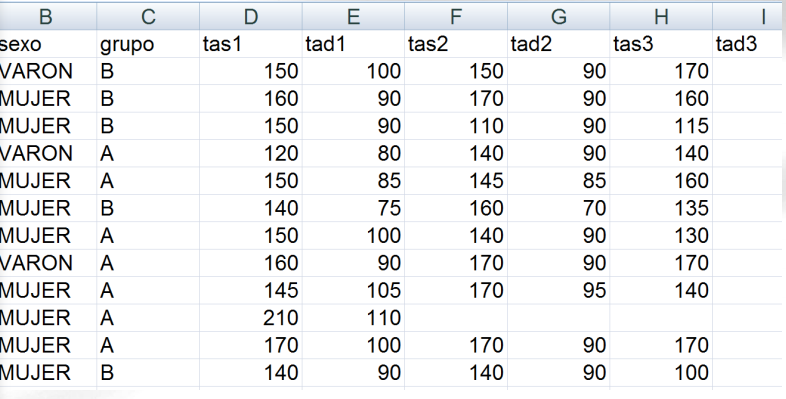
\includegraphics[width=0.9\linewidth,height=0.9\textheight]{images/ExampleDataHTA} \end{figure}
\end{frame}

\begin{frame}[fragile]{Introductory Example (2)}
\protect\hypertarget{introductory-example-2}{}
\begin{Shaded}
\begin{Highlighting}[]
\NormalTok{hta }\OtherTok{\textless{}{-}} \FunctionTok{read\_excel}\NormalTok{(}\StringTok{"datasets/hta.xls"}\NormalTok{)}
\FunctionTok{print}\NormalTok{(}\FunctionTok{head}\NormalTok{(hta))}
\end{Highlighting}
\end{Shaded}

\begin{verbatim}
## # A tibble: 6 x 27
##   numero sexo  grupo  tas1  tad1  tas2  tad2  tas3  tad3  tas4  tad4  tas5  tad5
##    <dbl> <chr> <chr> <dbl> <dbl> <dbl> <dbl> <dbl> <dbl> <dbl> <dbl> <dbl> <dbl>
## 1      1 VARON B       150   100   150    90   170    90   175    85   140    90
## 2      2 MUJER B       160    90   170    90   160    80   150    90   150    90
## 3      3 MUJER B       150    90   110    90   115    90   120    80   125    85
## 4      4 VARON A       120    80   140    90   140    90   130    90   130    95
## 5      5 MUJER A       150    85   145    85   160    90   140    80   120    80
## 6      6 MUJER B       140    75   160    70   135    75   140    70   140    75
## # ... with 14 more variables: tas6 <dbl>, tad6 <dbl>, tas7 <dbl>, tad7 <dbl>,
## #   tas8 <dbl>, tad8 <dbl>, tas9 <dbl>, tad9 <dbl>, tas10 <dbl>, tad10 <dbl>,
## #   tas11 <dbl>, tad11 <dbl>, tas12 <dbl>, tad12 <dbl>
\end{verbatim}
\end{frame}

\begin{frame}{Some questions to be answered}
\protect\hypertarget{some-questions-to-be-answered}{}
\begin{itemize}
\tightlist
\item
  Is diastolic (min) tension above 90, ``on average'', at the beginning
  of the study?
\item
  Are samples at baseline equivalent? -- In Age? Sex\%? Sist? Diast?
\item
  Has there been a change in BP between month 1 (first measure) and
  month 12?
\item
  Has this change been different between treatment groups?
\end{itemize}
\end{frame}

\begin{frame}{What type of test for each question?}
\protect\hypertarget{what-type-of-test-for-each-question}{}
\begin{itemize}
\item
  Is diastolic (min) tension above 90, ``on average'', at the beginning
  of the study?

  -- \emph{One variable. Test about the mean}
\item
  Are samples at baseline equivalent?

  -- \emph{Comparison between distinct groups of individuals in two
  groups (A/B, Male/Fem)}
\item
  Has there been a change in BP between month 1 (first measure) and
  month 12?

  -- \emph{Comparison between same individuals at different time points}
\end{itemize}
\end{frame}

\begin{frame}[fragile]{Always start looking at the data}
\protect\hypertarget{always-start-looking-at-the-data}{}
\begin{Shaded}
\begin{Highlighting}[]
\FunctionTok{par}\NormalTok{(}\AttributeTok{mfrow=}\FunctionTok{c}\NormalTok{(}\DecValTok{1}\NormalTok{,}\DecValTok{2}\NormalTok{)) }\CommentTok{\# Draw four plots in one panel }
\FunctionTok{with}\NormalTok{(hta, }\FunctionTok{boxplot}\NormalTok{(tad1, }\AttributeTok{main=}\StringTok{"Box{-}plot"}\NormalTok{) )}
\FunctionTok{with}\NormalTok{(hta, }\FunctionTok{hist}\NormalTok{(tad1) )}
\end{Highlighting}
\end{Shaded}

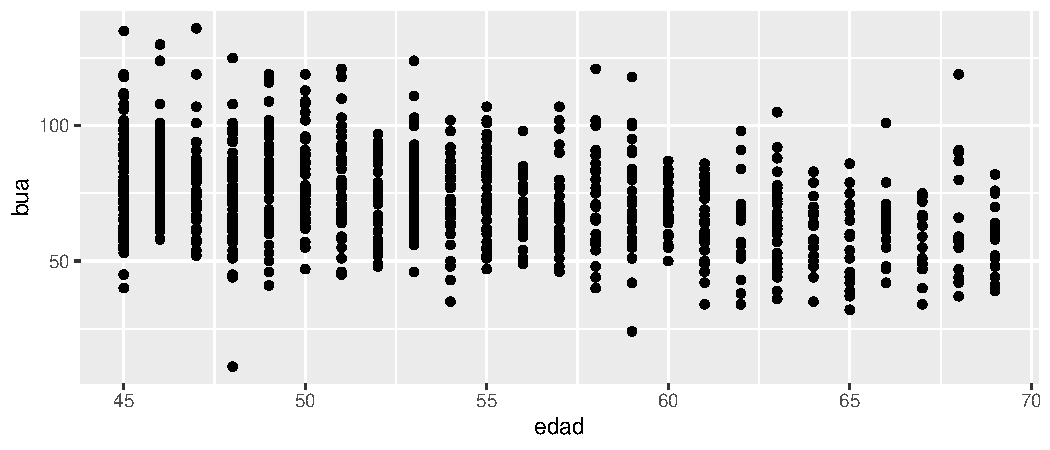
\includegraphics[width=0.9\linewidth,height=0.9\textheight]{StatisticsWithR-7-8-Tests_with_continuous-categorical_variables_files/figure-beamer/unnamed-chunk-4-1}

\begin{Shaded}
\begin{Highlighting}[]
\FunctionTok{par}\NormalTok{(}\AttributeTok{mfrow=}\FunctionTok{c}\NormalTok{(}\DecValTok{1}\NormalTok{,}\DecValTok{1}\NormalTok{)) }\CommentTok{\# Back to one plot per panel}
\end{Highlighting}
\end{Shaded}
\end{frame}

\begin{frame}{General approach}
\protect\hypertarget{general-approach}{}
\begin{itemize}
\item
  Hypothesis tesing is useful to answer some questions in problems.
\item
  These can be applied in distinct scenarios:

  \begin{itemize}
  \tightlist
  \item
    With numerical/continuos or categorical variables.
  \item
    With data distribued as a gaussian population or not
  \item
    With one or more groups of data.
  \item
    With dependent or independent data.
  \end{itemize}
\item
  Try not to blindly apply recipes

  \begin{itemize}
  \tightlist
  \item
    Think about the situation that generated the data
  \item
    Think about how your question becomes a test
  \item
    Think about the assumptions of the test, how to check them and how
    robust may the test be to assumption violations.
  \item
    Know how to apply the test
  \item
    Do not blindly and dumby rely on cutoffs!
  \end{itemize}
\end{itemize}
\end{frame}

\begin{frame}[fragile]{Normality Test}
\protect\hypertarget{normality-test}{}
\begin{figure}
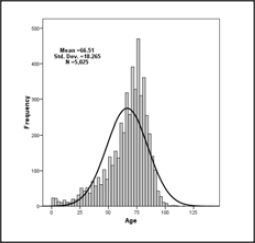
\includegraphics[width=0.8\linewidth]{images/normalityplot} \end{figure}

\small

\begin{Shaded}
\begin{Highlighting}[]
\FunctionTok{with}\NormalTok{(hta,}\FunctionTok{shapiro.test}\NormalTok{(tad1) ) }\CommentTok{\# Shapiro Wilk test}
\end{Highlighting}
\end{Shaded}

\begin{verbatim}
## 
##  Shapiro-Wilk normality test
## 
## data:  tad1
## W = 0.96622, p-value = 0.09512
\end{verbatim}
\end{frame}

\begin{frame}{One sample Test}
\protect\hypertarget{one-sample-test}{}
\begin{itemize}
\item
  We do not use it very often.
\item
  Very similar to estimation questions. It can be solved calculating a
  confidence interval
\item
  Idea: We want to verify from a sample a previous hypothesis about the
  mean in a population
\item
  Example: \emph{Can it be accepted that the initial TAD is 90 or
  greater in hypertensive patients?}
\item
  If data is assumed to follow a normal distribution: \emph{t-test}
\item
  If data is \textbf{not} assumed to follow a normal distribution:
  \emph{wilcoxon-tets}
\end{itemize}
\end{frame}

\begin{frame}[fragile]{Example of one-sample test}
\protect\hypertarget{example-of-one-sample-test}{}
Assuming data does not follow a normal distribution \ldots{}

\tiny

\begin{Shaded}
\begin{Highlighting}[]
\FunctionTok{with}\NormalTok{(hta,}\FunctionTok{wilcox.test}\NormalTok{(tad1,}\AttributeTok{mu=}\DecValTok{90}\NormalTok{) ) }\CommentTok{\# One sample wilcoxon.test}
\end{Highlighting}
\end{Shaded}

\begin{verbatim}
## 
##  Wilcoxon signed rank test with continuity correction
## 
## data:  tad1
## V = 429, p-value = 0.2173
## alternative hypothesis: true location is not equal to 90
\end{verbatim}

The t-test is robust to small departures of normality \ldots{}

\tiny

\begin{Shaded}
\begin{Highlighting}[]
\FunctionTok{with}\NormalTok{(hta,}\FunctionTok{t.test}\NormalTok{(tad1,}\AttributeTok{mu=}\DecValTok{90}\NormalTok{) ) }\CommentTok{\# One sample T.test}
\end{Highlighting}
\end{Shaded}

\begin{verbatim}
## 
##  One Sample t-test
## 
## data:  tad1
## t = -1.2137, df = 59, p-value = 0.2297
## alternative hypothesis: true mean is not equal to 90
## 95 percent confidence interval:
##  85.80626 91.02707
## sample estimates:
## mean of x 
##  88.41667
\end{verbatim}
\end{frame}

\begin{frame}{Exercise 1}
\protect\hypertarget{exercise-1}{}
\begin{enumerate}
\tightlist
\item
  Check the normality of tas1 variable, call it ``TAS'' in hta dataset
\item
  Can it be accepted that the initial TAS is 120 in Hipertensive
  patients?
\item
  Find the 95\% confidence interval for the mean of tas1 variable
\item
  Extra: Can it be accepted that the initial TAS is higher than 120 in
  Hipertensive women?
\end{enumerate}
\end{frame}

\begin{frame}{Comparison between two groups (``two-sample problems'')}
\protect\hypertarget{comparison-between-two-groups-two-sample-problems}{}
\begin{itemize}
\item
  Most of the times, tests are associated with comparison between two or
  more groups.

  \begin{itemize}
  \tightlist
  \item
    Are the two groups A and B comparable?, that is, given a certain
    variable, does it take on average, the same value, at baseline time?
  \item
    Is blood pressure comparable between first and 12th measures?
  \end{itemize}
\end{itemize}

Notice that:

\begin{itemize}
\tightlist
\item
  the first question implies comparison between distinct groups of
  individuals
\item
  while the first one assumes comparison between the same individuals at
  two time points.
\end{itemize}
\end{frame}

\begin{frame}[fragile]{Start looking at the data}
\protect\hypertarget{start-looking-at-the-data}{}
\begin{Shaded}
\begin{Highlighting}[]
\FunctionTok{with}\NormalTok{(hta, }\FunctionTok{boxplot}\NormalTok{(tad1}\SpecialCharTok{\textasciitilde{}}\NormalTok{grupo))}
\end{Highlighting}
\end{Shaded}

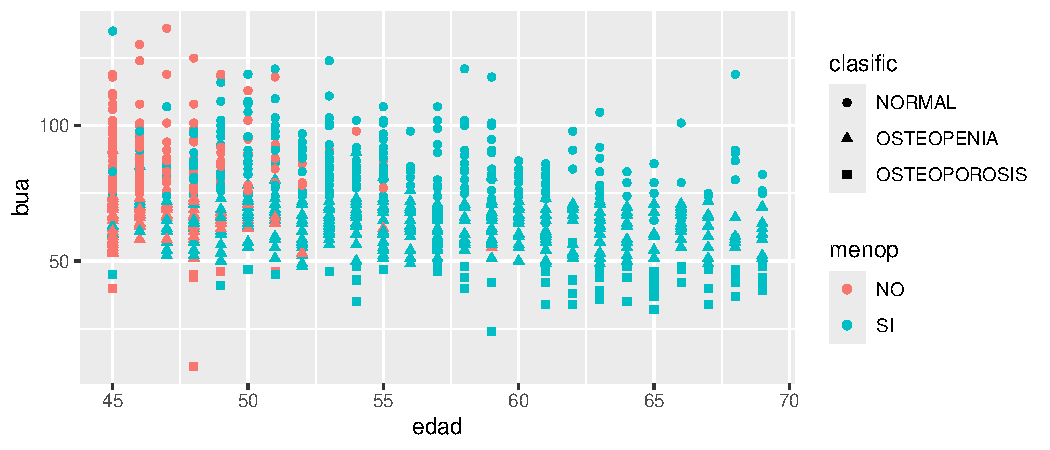
\includegraphics{StatisticsWithR-7-8-Tests_with_continuous-categorical_variables_files/figure-beamer/unnamed-chunk-6-1.pdf}
\end{frame}

\begin{frame}[fragile]{Compare two groups assuming normality:}
\protect\hypertarget{compare-two-groups-assuming-normality}{}
\begin{block}{two sample t-test for independent groups}
\protect\hypertarget{two-sample-t-test-for-independent-groups}{}
\begin{itemize}
\item
  The two-sample t-test is used to compàre two groups assuming
  normality.
\item
  The test changes depending on if the variances of the two groups can
  be considered equal or not.

  \begin{itemize}
  \tightlist
  \item
    This preliminary comparison is omitted here.
  \end{itemize}
\end{itemize}

\tiny

\begin{Shaded}
\begin{Highlighting}[]
\FunctionTok{with}\NormalTok{(hta,}\FunctionTok{t.test}\NormalTok{(tad1}\SpecialCharTok{\textasciitilde{}}\FunctionTok{factor}\NormalTok{(sexo),}\AttributeTok{var.equal=}\ConstantTok{FALSE}\NormalTok{ ))}
\end{Highlighting}
\end{Shaded}

\begin{verbatim}
## 
##  Welch Two Sample t-test
## 
## data:  tad1 by factor(sexo)
## t = 0.33362, df = 38.144, p-value = 0.7405
## alternative hypothesis: true difference in means between group MUJER and group VARON is not equal to 0
## 95 percent confidence interval:
##  -4.852834  6.768228
## sample estimates:
## mean in group MUJER mean in group VARON 
##            88.78378            87.82609
\end{verbatim}
\end{block}
\end{frame}

\begin{frame}[fragile]{Compare two groups without assuming normality}
\protect\hypertarget{compare-two-groups-without-assuming-normality}{}
\begin{block}{U Mann-Whitney or Sum Rank non parametric test}
\protect\hypertarget{u-mann-whitney-or-sum-rank-non-parametric-test}{}
\tiny

\begin{Shaded}
\begin{Highlighting}[]
\NormalTok{hta}\SpecialCharTok{\%\textgreater{}\%} 
  \FunctionTok{group\_by}\NormalTok{(grupo) }\SpecialCharTok{\%\textgreater{}\%} 
  \FunctionTok{summarise}\NormalTok{(}\AttributeTok{median =} \FunctionTok{median}\NormalTok{(tad1)) }
\end{Highlighting}
\end{Shaded}

\begin{verbatim}
## # A tibble: 2 x 2
##   grupo median
##   <chr>  <dbl>
## 1 A         85
## 2 B         90
\end{verbatim}

\begin{Shaded}
\begin{Highlighting}[]
\FunctionTok{with}\NormalTok{(hta,}\FunctionTok{wilcox.test}\NormalTok{(tad1}\SpecialCharTok{\textasciitilde{}}\FunctionTok{factor}\NormalTok{(grupo)}
\NormalTok{    ,}\AttributeTok{alternative=}\StringTok{\textquotesingle{}two.sided\textquotesingle{}}\NormalTok{,}\AttributeTok{exact=}\ConstantTok{TRUE}\NormalTok{, }\AttributeTok{correct=}\ConstantTok{FALSE}\NormalTok{))}
\end{Highlighting}
\end{Shaded}

\begin{verbatim}
## 
##  Wilcoxon rank sum test
## 
## data:  tad1 by factor(grupo)
## W = 432, p-value = 0.7926
## alternative hypothesis: true location shift is not equal to 0
\end{verbatim}

\begin{itemize}
\tightlist
\item
  Null Hypothesis cannot be rejected
\end{itemize}
\end{block}
\end{frame}

\begin{frame}{Exercise 2}
\protect\hypertarget{exercise-2}{}
\begin{enumerate}
\tightlist
\item
  Is Diastolic pressure (``TDA'') comparable at baseline time between
  Men and women?
\item
  What is the Hypothesis that we want to test? Describe the null
  hypothesis and the alternative hypothesis.
\item
  What test would be appropiate to answer the question?
\item
  Compute and decide
\item
  Apply a non-parametric test and compare the results
\end{enumerate}
\end{frame}

\begin{frame}{Comparisons with dependent (paired) data}
\protect\hypertarget{comparisons-with-dependent-paired-data}{}
\begin{itemize}
\item
  If we consider two groups of dependent data we are in a prticular
  situation.

  \begin{itemize}
  \tightlist
  \item
    Apparently two groups
  \item
    Only one group of individuals
  \end{itemize}
\item
  Computer programs usually provide tests for ``paired data'', but they
  are essentially one-sample tests fro the difference between the values
  of the same individuals.
\item
  Again, depending on, if normality is assumed or not, we rely on
  \emph{paired-t-test} or \emph{wilcoxon test for paired data}.
\end{itemize}
\end{frame}

\begin{frame}{Exercise 3}
\protect\hypertarget{exercise-3}{}
\begin{itemize}
\tightlist
\item
  Can we consider that systolic and diastolic pressure have changed
  between baseline and month 12?
\item
  Choose the appropriate test and apply it to yioeld a decision.
\item
  Think carefully about the hypothesis being tested.

  \begin{itemize}
  \tightlist
  \item
    What is a reasonable option for the alternative hypothesis?
  \end{itemize}
\end{itemize}
\end{frame}

\begin{frame}[fragile]{Categorical Variables}
\protect\hypertarget{categorical-variables}{}
\begin{itemize}
\item
  Categorical variables represent facts that can be better described
  with \emph{labels} than with numbers.

  \begin{itemize}
  \tightlist
  \item
    Example: \texttt{Sex}, better choose from \{\texttt{Male} ,
    \texttt{Female}\} than from: \{1,2\}.
  \end{itemize}
\item
  Sometimes ordering of labels makes sense, although \emph{it is not
  reasonable to assign numbers to categories}:

  \begin{itemize}
  \item
    Example: \texttt{Tumor\ stage}: \{1,2,3,4\}, but \(1+2\neq 3\)!!!
  \item
    \texttt{Sex} is an example of a categorical variable in
    \texttt{nominal} scale
  \item
    \texttt{Stage} is an example of a categorical variable in
    \texttt{ordinal} scale
  \end{itemize}
\end{itemize}
\end{frame}

\begin{frame}[fragile]{Representing categorical variables in R}
\protect\hypertarget{representing-categorical-variables-in-r}{}
\begin{itemize}
\tightlist
\item
  Categorical variables are well represented with \emph{factors}
\end{itemize}

\begin{Shaded}
\begin{Highlighting}[]
\NormalTok{sex }\OtherTok{\textless{}{-}} \FunctionTok{factor}\NormalTok{(}\FunctionTok{c}\NormalTok{(}\StringTok{"Female"}\NormalTok{, }\StringTok{"Male"}\NormalTok{))}
\NormalTok{blood\_group }\OtherTok{\textless{}{-}} \FunctionTok{factor}\NormalTok{(}\FunctionTok{c}\NormalTok{(}\StringTok{"A"}\NormalTok{, }\StringTok{"B"}\NormalTok{, }\StringTok{"AB"}\NormalTok{, }\StringTok{"O"}\NormalTok{))}
\end{Highlighting}
\end{Shaded}

\begin{itemize}
\tightlist
\item
  Be careful with the names of factors, by default, \emph{levels}
  assigned in alphabetical order.
\end{itemize}

\begin{Shaded}
\begin{Highlighting}[]
\FunctionTok{levels}\NormalTok{(blood\_group)}
\end{Highlighting}
\end{Shaded}

\begin{verbatim}
## [1] "A"  "AB" "B"  "O"
\end{verbatim}

\begin{itemize}
\tightlist
\item
  To verify class of a variable
\end{itemize}

\begin{Shaded}
\begin{Highlighting}[]
\FunctionTok{class}\NormalTok{(sex)}
\end{Highlighting}
\end{Shaded}

\begin{verbatim}
## [1] "factor"
\end{verbatim}
\end{frame}

\begin{frame}[fragile]{Creating factors}
\protect\hypertarget{creating-factors}{}
\begin{itemize}
\item
  Factors can be created \ldots{}

  \begin{itemize}
  \item
    automatically, when reading a file or

    \begin{itemize}
    \tightlist
    \item
      Not all functions for reading data from file will create a
      factor!!!
    \item
      Usually levels will be defined from alphabetic order
    \end{itemize}
  \item
    using the \texttt{factor} or the \texttt{as.factor} commands.

    \begin{itemize}
    \tightlist
    \item
      more flexible
    \end{itemize}
  \end{itemize}
\end{itemize}
\end{frame}

\begin{frame}[fragile]{Create factors automatically}
\protect\hypertarget{create-factors-automatically}{}
\begin{itemize}
\item
  This is achieved by

  \begin{itemize}
  \item
    Using the \texttt{read.table} or \texttt{read.delim} functions for
    reading

    \begin{itemize}
    \tightlist
    \item
      Setting the ``character variables as.factors'' to TRUE
    \end{itemize}
  \end{itemize}
\item
  Example

  \begin{itemize}
  \tightlist
  \item
    Load the \texttt{diabetes} dataset using the
    \texttt{Import\ Dataset} feature of Rstudio

    \begin{itemize}
    \tightlist
    \item
      From text (base) (use the file \texttt{osteoporosis.csv})
    \item
      From text (readr) (use the file \texttt{osteoporosis.csv})
    \end{itemize}
  \item
    What is the class of the variable \texttt{menop}
  \end{itemize}
\end{itemize}
\end{frame}

\begin{frame}[fragile]{Create factors automatically}
\protect\hypertarget{create-factors-automatically-1}{}
\begin{Shaded}
\begin{Highlighting}[]
\NormalTok{osteo1 }\OtherTok{\textless{}{-}} \FunctionTok{read.csv}\NormalTok{(}\StringTok{"datasets/osteoporosis.csv"}\NormalTok{,}\AttributeTok{sep =} \StringTok{"}\SpecialCharTok{\textbackslash{}t}\StringTok{"}\NormalTok{,}
                   \AttributeTok{stringsAsFactors=}\ConstantTok{TRUE}\NormalTok{)}
\FunctionTok{class}\NormalTok{(osteo1}\SpecialCharTok{$}\NormalTok{menop)}
\FunctionTok{summary}\NormalTok{(osteo1}\SpecialCharTok{$}\NormalTok{menop)}
\FunctionTok{str}\NormalTok{(osteo1)}

\FunctionTok{library}\NormalTok{(readr)}
\NormalTok{osteo2 }\OtherTok{\textless{}{-}} \FunctionTok{read\_delim}\NormalTok{(}\StringTok{"datasets/osteoporosis.csv"}\NormalTok{, }\StringTok{"}\SpecialCharTok{\textbackslash{}t}\StringTok{"}\NormalTok{, }
                     \AttributeTok{escape\_double =} \ConstantTok{FALSE}\NormalTok{)}
\FunctionTok{class}\NormalTok{(osteo2}\SpecialCharTok{$}\NormalTok{menop)}
\NormalTok{osteo2}\SpecialCharTok{$}\NormalTok{menop }\OtherTok{\textless{}{-}} \FunctionTok{as.factor}\NormalTok{(osteo2}\SpecialCharTok{$}\NormalTok{menop)}
\FunctionTok{class}\NormalTok{(osteo2}\SpecialCharTok{$}\NormalTok{menop)}
\FunctionTok{summary}\NormalTok{(osteo2}\SpecialCharTok{$}\NormalTok{menop)}
\FunctionTok{str}\NormalTok{(osteo2)}
\end{Highlighting}
\end{Shaded}
\end{frame}

\begin{frame}[fragile]{Exercise 4}
\protect\hypertarget{exercise-4}{}
\begin{itemize}
\item
  Select \texttt{diabetes.xls} datasets
\item
  Read the dataset into R and check that the categorical variables you
  are interested (mort, tabac, ecg) in are converted into factors.
\item
  Confirm the conversion by summarizing the variables
\end{itemize}
\end{frame}

\begin{frame}{The analysis of categorical variables}
\protect\hypertarget{the-analysis-of-categorical-variables}{}
\begin{itemize}
\item
  The analysis of categorical data proceeds as usual:
\item
  Start exploring the data with the tables and graphics
\item
  Proceed to estimation and/or testing if \emph{appropriate}
\item
  Estimation

  \begin{itemize}
  \tightlist
  \item
    Proportions: Point estimates, confidence intervals
  \end{itemize}
\item
  Testing

  \begin{itemize}
  \tightlist
  \item
    One variable (tests with proportions)
  \item
    With two variables (chi-square and related)
  \end{itemize}
\end{itemize}
\end{frame}

\begin{frame}{Types of test with categorical variables}
\protect\hypertarget{types-of-test-with-categorical-variables}{}
\begin{itemize}
\item
  One variable (tests with proportions)

  \begin{itemize}
  \tightlist
  \item
    Does the proportion (\% affected) match a given value?
  \item
    Is the proportion (\% affected) the same in two populations?
  \end{itemize}
\item
  With two variables (chi-square and related)

  \begin{itemize}
  \tightlist
  \item
    Is there an association between two categorical variables?
  \item
    Is there a relationship between the values of a categorical variable
    before and after treatment?
  \end{itemize}
\end{itemize}
\end{frame}

\begin{frame}{Select the test according to each situation (3)}
\protect\hypertarget{select-the-test-according-to-each-situation-3}{}
\begin{block}{Some test options when variables are categorical}
\protect\hypertarget{some-test-options-when-variables-are-categorical}{}
\begin{figure}
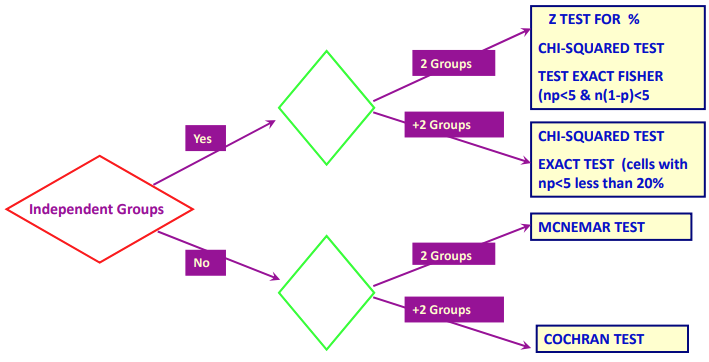
\includegraphics[width=0.9\linewidth,height=0.9\textheight]{images/tests4categoricalVariables} \end{figure}
\end{block}
\end{frame}

\begin{frame}{Example}
\protect\hypertarget{example}{}
Consider the following study relating smoking and cancer.

\begin{figure}
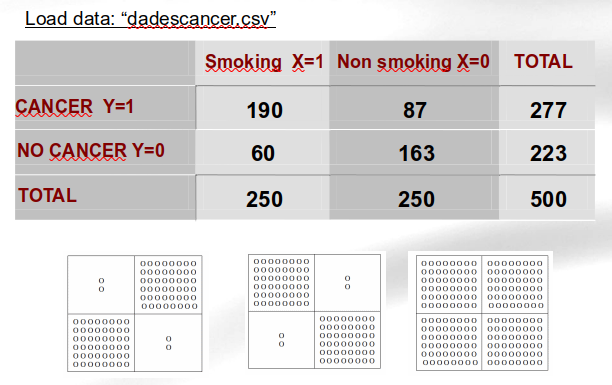
\includegraphics[width=0.8\linewidth]{images/cancerAndSmoking1png} \end{figure}

Our goal here would be to determine if there is an association between
smoking and cancer.
\end{frame}

\begin{frame}[fragile]{Crosstabulating a dataset}
\protect\hypertarget{crosstabulating-a-dataset}{}
\begin{itemize}
\item
  Data may come from a table (aggregated) or disagregated in a data
  file.
\item
  In this case we need to build the table applying ``cross-tabulation''
\end{itemize}

\begin{Shaded}
\begin{Highlighting}[]
\NormalTok{dadescancer }\OtherTok{\textless{}{-}} \FunctionTok{read.csv}\NormalTok{(}\StringTok{"datasets/dadescancer.csv"}\NormalTok{, }
                        \AttributeTok{stringsAsFactors =} \ConstantTok{TRUE}\NormalTok{)}
\end{Highlighting}
\end{Shaded}

\begin{Shaded}
\begin{Highlighting}[]
\CommentTok{\#attach(dadescancer)}
\NormalTok{mytable }\OtherTok{\textless{}{-}}\FunctionTok{table}\NormalTok{(dadescancer}\SpecialCharTok{$}\NormalTok{cancer, dadescancer}\SpecialCharTok{$}\NormalTok{fumar)}
\NormalTok{mytable}
\end{Highlighting}
\end{Shaded}

\begin{verbatim}
##            
##             Fuma No fuma
##   Cancer     190      87
##   No cancer   60     163
\end{verbatim}
\end{frame}

\begin{frame}[fragile]{Crosstabulation (2): Marginal tables}
\protect\hypertarget{crosstabulation-2-marginal-tables}{}
Marginal values are important to understand the structure of the data:

\begin{Shaded}
\begin{Highlighting}[]
\NormalTok{mytable}\OtherTok{\textless{}{-}} \FunctionTok{addmargins}\NormalTok{(mytable)}
\NormalTok{mytable}
\end{Highlighting}
\end{Shaded}

\begin{verbatim}
##            
##             Fuma No fuma Sum
##   Cancer     190      87 277
##   No cancer   60     163 223
##   Sum        250     250 500
\end{verbatim}
\end{frame}

\begin{frame}[fragile]{Crosstabulation (3): In percentages}
\protect\hypertarget{crosstabulation-3-in-percentages}{}
Showing tables as percentages is useful for comparisons

\begin{Shaded}
\begin{Highlighting}[]
\FunctionTok{prop.table}\NormalTok{(mytable) }\CommentTok{\# cell percentages}
\end{Highlighting}
\end{Shaded}

\begin{verbatim}
##            
##               Fuma No fuma    Sum
##   Cancer    0.0950  0.0435 0.1385
##   No cancer 0.0300  0.0815 0.1115
##   Sum       0.1250  0.1250 0.2500
\end{verbatim}

\begin{Shaded}
\begin{Highlighting}[]
\FunctionTok{prop.table}\NormalTok{(mytable, }\DecValTok{1}\NormalTok{) }\CommentTok{\# row percentages}
\end{Highlighting}
\end{Shaded}

\begin{verbatim}
##            
##                  Fuma   No fuma       Sum
##   Cancer    0.3429603 0.1570397 0.5000000
##   No cancer 0.1345291 0.3654709 0.5000000
##   Sum       0.2500000 0.2500000 0.5000000
\end{verbatim}

\begin{Shaded}
\begin{Highlighting}[]
\CommentTok{\# prop.table(mytable, 2) \# column percentages}
\end{Highlighting}
\end{Shaded}
\end{frame}

\begin{frame}{Exercise 5}
\protect\hypertarget{exercise-5}{}
\begin{itemize}
\tightlist
\item
  With the diabetes dataset repeat the crosstabulation done above using

  \begin{itemize}
  \tightlist
  \item
    Two categorical variables
  \item
    Variable ``mort'' and a newly created variable ``bmi30'' created by
    properly categorizing variable bmi.
  \end{itemize}
\end{itemize}
\end{frame}

\begin{frame}{One variable: Proportion tests}
\protect\hypertarget{one-variable-proportion-tests}{}
\begin{itemize}
\item
  According to medical literature, in the period 1950-1980, the
  proportion of obese individuals (defined as: BMI \(\geq 30\)) was 15\%
  in the population of men over 55 years old.
\item
  A random sample obtained from the same population between 2000 and
  2003 showed that, over a total of 723 men older than 55, 142 were
  obese.
\item
  With a significance level of 5\%, can we say that the population of
  men older than 55 in 2000-2003 had the same proportion of obese cases
  than that population had in 50'-80'?
\end{itemize}
\end{frame}

\begin{frame}[fragile]{Proportion tests with R}
\protect\hypertarget{proportion-tests-with-r}{}
Alternative ``NOT EQUAL''. This is set by default.

\begin{Shaded}
\begin{Highlighting}[]
\FunctionTok{prop.test}\NormalTok{(}\AttributeTok{x=}\DecValTok{142}\NormalTok{, }\AttributeTok{n=}\DecValTok{723}\NormalTok{, }\AttributeTok{p=}\FloatTok{0.15}\NormalTok{)}
\end{Highlighting}
\end{Shaded}

\begin{verbatim}
## 
##  1-sample proportions test with continuity correction
## 
## data:  142 out of 723, null probability 0.15
## X-squared = 11.849, df = 1, p-value = 0.0005768
## alternative hypothesis: true p is not equal to 0.15
## 95 percent confidence interval:
##  0.1684325 0.2276606
## sample estimates:
##         p 
## 0.1964039
\end{verbatim}
\end{frame}

\begin{frame}[fragile]
Alternative ``GREATER''

\begin{Shaded}
\begin{Highlighting}[]
\FunctionTok{prop.test}\NormalTok{(}\AttributeTok{x=}\DecValTok{142}\NormalTok{, }\AttributeTok{n=}\DecValTok{723}\NormalTok{, }\AttributeTok{p=}\FloatTok{0.15}\NormalTok{, }\AttributeTok{alternative=}\StringTok{"g"}\NormalTok{)}
\end{Highlighting}
\end{Shaded}

\begin{verbatim}
## 
##  1-sample proportions test with continuity correction
## 
## data:  142 out of 723, null probability 0.15
## X-squared = 11.849, df = 1, p-value = 0.0002884
## alternative hypothesis: true p is greater than 0.15
## 95 percent confidence interval:
##  0.1725953 1.0000000
## sample estimates:
##         p 
## 0.1964039
\end{verbatim}
\end{frame}

\begin{frame}[fragile]
Alternative ``LESS THAN''

\begin{Shaded}
\begin{Highlighting}[]
\FunctionTok{prop.test}\NormalTok{(}\AttributeTok{x=}\DecValTok{142}\NormalTok{, }\AttributeTok{n=}\DecValTok{723}\NormalTok{, }\AttributeTok{p=}\FloatTok{0.15}\NormalTok{, }\AttributeTok{alternative=}\StringTok{"l"}\NormalTok{)}
\end{Highlighting}
\end{Shaded}

\begin{verbatim}
## 
##  1-sample proportions test with continuity correction
## 
## data:  142 out of 723, null probability 0.15
## X-squared = 11.849, df = 1, p-value = 0.9997
## alternative hypothesis: true p is less than 0.15
## 95 percent confidence interval:
##  0.0000000 0.2225404
## sample estimates:
##         p 
## 0.1964039
\end{verbatim}

Notice that \emph{choosing the wrong alternative may yield unreasonable
conclusions}.
\end{frame}

\begin{frame}[fragile]{Estimation comes with proportion test}
\protect\hypertarget{estimation-comes-with-proportion-test}{}
\begin{itemize}
\item
  \texttt{prop.test} does \textbf{three} distinct calculations

  \begin{itemize}
  \tightlist
  \item
    A test for the hypothesis \(H_0: p=p_0\) is performed
  \item
    A confidence interval for \(p\) is built based on the sample
  \item
    A point estimate for \(p\) is also provided.
  \end{itemize}
\end{itemize}

\begin{figure}
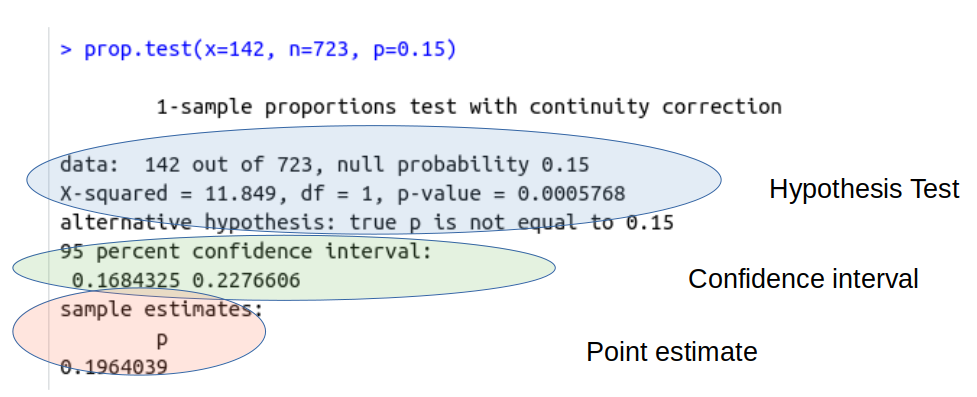
\includegraphics[width=1\linewidth]{images/propTestsAndCI} \end{figure}
\end{frame}

\begin{frame}[fragile]{Exercise 3}
\protect\hypertarget{exercise-3-1}{}
\begin{itemize}
\item
  In the diabetes dataset.

  \begin{itemize}
  \tightlist
  \item
    Test the hypothesis that the proportion of patients with
    \texttt{bmi30} is higher than 40\%

    \begin{itemize}
    \tightlist
    \item
      In the global population of the study
    \item
      Only in patients with `mort' equal ``Muerto''
    \end{itemize}
  \end{itemize}
\end{itemize}
\end{frame}

\begin{frame}{Contingency tables}
\protect\hypertarget{contingency-tables}{}
\begin{itemize}
\item
  A contingency table (a.k.a cross tabulation or cross tab) is a
  matrix-like table that displays the (multivariate) frequency
  distribution of the variables.
\item
  It is bidimensional, and classifies all observations according to two
  categorical variables (A and B, rows and columns).
\end{itemize}

\begin{figure}
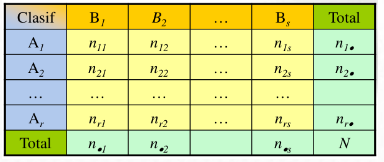
\includegraphics[width=0.8\linewidth]{images/contingencytables1} \end{figure}
\end{frame}

\begin{frame}{Chi-squared test}
\protect\hypertarget{chi-squared-test}{}
\begin{itemize}
\tightlist
\item
  A \emph{familiy} of tests receiving its name because they all rely on
  the \emph{Chi-Squared distribution} to compute the test probabilities.
\end{itemize}

\textbf{Chi squared independence test}

\begin{itemize}
\tightlist
\item
  When the sample comes from a single population with 2 categorical
  variables, the aim is to determine if there is relationship between
  them.
\end{itemize}

\textbf{Chi squared homogeneity test}

\begin{itemize}
\tightlist
\item
  When each row is a sample from distinct populations (groups,
  subgroups\ldots), the aim is to determine if both groups have
  significative differences in that variable
\end{itemize}
\end{frame}

\begin{frame}{Chi-squared tests}
\protect\hypertarget{chi-squared-tests}{}
\begin{itemize}
\item
  When we have:

  \begin{itemize}
  \tightlist
  \item
    quantitative data,
  \item
    two or more categories,
  \item
    independent observations,
  \item
    adequate sample size (\textgreater10)
  \end{itemize}
\item
  and our questions are like\ldots{}

  \begin{itemize}
  \item
    \emph{Do the number of individuals or objects that fall in each pair
    of categories differ significantly from the number you would expect
    if there was no association?}
  \item
    \emph{Is this difference between the expected and observed due to
    chance (``sampling variation''), or is it a real difference?}
  \end{itemize}
\end{itemize}
\end{frame}

\begin{frame}{Chi squared.test: Observed vs expected}
\protect\hypertarget{chi-squared.test-observed-vs-expected}{}
\begin{figure}
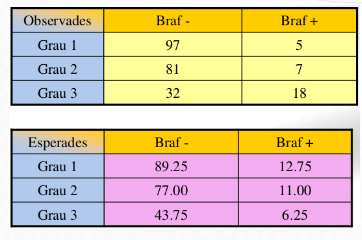
\includegraphics[width=0.8\linewidth]{images/observedvsexpected} \end{figure}
\end{frame}

\begin{frame}[fragile]{Chi squared tests: Observed vs expected with R}
\protect\hypertarget{chi-squared-tests-observed-vs-expected-with-r}{}
\begin{Shaded}
\begin{Highlighting}[]
\FunctionTok{require}\NormalTok{(gmodels)}
\NormalTok{mytable }\OtherTok{\textless{}{-}} \FunctionTok{table}\NormalTok{(dadescancer}\SpecialCharTok{$}\NormalTok{cancer, dadescancer}\SpecialCharTok{$}\NormalTok{fumar)}
\FunctionTok{CrossTable}\NormalTok{(mytable,}\AttributeTok{expected =}\NormalTok{ T,}\AttributeTok{prop.chisq =}\NormalTok{ F,}\AttributeTok{prop.c =}\NormalTok{ F,}\AttributeTok{prop.r =}\NormalTok{ F)}
\end{Highlighting}
\end{Shaded}

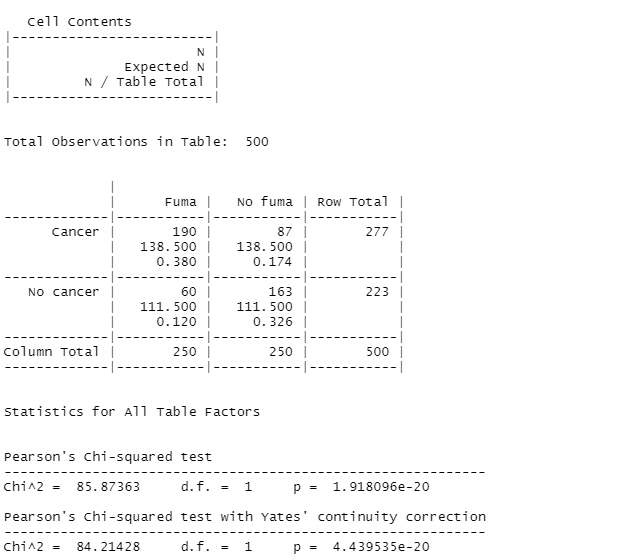
\includegraphics{images/chi.PNG}
\end{frame}

\begin{frame}[fragile]{Chi squared tests with R}
\protect\hypertarget{chi-squared-tests-with-r}{}
\begin{Shaded}
\begin{Highlighting}[]
\FunctionTok{chisq.test}\NormalTok{ (mytable)}
\end{Highlighting}
\end{Shaded}

\begin{verbatim}
## 
##  Pearson's Chi-squared test with Yates' continuity correction
## 
## data:  mytable
## X-squared = 84.214, df = 1, p-value < 2.2e-16
\end{verbatim}
\end{frame}

\begin{frame}[fragile]{Fisher test. an assumptions-free alternative}
\protect\hypertarget{fisher-test.-an-assumptions-free-alternative}{}
Chi-squared test require that sample sizes are ``big'' and expected
frequencies are, at least greater than 5.

Fisher test can be an alternative if these assumptions are not met,
especially for two times two tables.

\begin{Shaded}
\begin{Highlighting}[]
\FunctionTok{fisher.test}\NormalTok{(mytable)}
\end{Highlighting}
\end{Shaded}

\begin{verbatim}
## 
##  Fisher's Exact Test for Count Data
## 
## data:  mytable
## p-value < 2.2e-16
## alternative hypothesis: true odds ratio is not equal to 1
## 95 percent confidence interval:
##  3.945907 8.936465
## sample estimates:
## odds ratio 
##   5.909114
\end{verbatim}
\end{frame}

\begin{frame}[fragile]{Exercise 6}
\protect\hypertarget{exercise-6}{}
\begin{itemize}
\item
  Use the diabetes dataset to study if it can be detected an association
  between the variables \texttt{mort} and \texttt{tabac} in the diabetes
  dataset.
\item
  Do not start with a test but with an appropriate summarization and
  visualization!
\end{itemize}
\end{frame}

\begin{frame}{Mcnemar test}
\protect\hypertarget{mcnemar-test}{}
Mcnemar test is used to compare the frequencies of paired samples of
dichotomous data

\begin{itemize}
\item
  Ho: There is no significant change in individuals after the treatment
\item
  H1: There is a significant change in individuals after the treatment
\end{itemize}
\end{frame}

\begin{frame}[fragile]{Mcnemar test. Example}
\protect\hypertarget{mcnemar-test.-example}{}
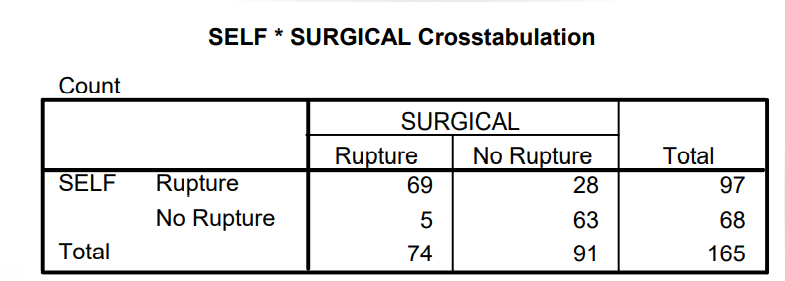
\includegraphics{images/mcnemar.PNG}

\begin{Shaded}
\begin{Highlighting}[]
\NormalTok{.Table }\OtherTok{\textless{}{-}} \FunctionTok{matrix}\NormalTok{(}\FunctionTok{c}\NormalTok{(}\DecValTok{69}\NormalTok{,}\DecValTok{28}\NormalTok{,}\DecValTok{5}\NormalTok{,}\DecValTok{63}\NormalTok{), }\DecValTok{2}\NormalTok{, }\DecValTok{2}\NormalTok{, }\AttributeTok{byrow=}\ConstantTok{TRUE}\NormalTok{)}
\FunctionTok{mcnemar.test}\NormalTok{(.Table)}
\end{Highlighting}
\end{Shaded}

\begin{verbatim}
## 
##  McNemar's Chi-squared test with continuity correction
## 
## data:  .Table
## McNemar's chi-squared = 14.667, df = 1, p-value = 0.0001283
\end{verbatim}
\end{frame}

\end{document}
